\documentclass{standalone}
\usepackage{tikz}
\usetikzlibrary{positioning, shapes.geometric, calc}

\begin{document}

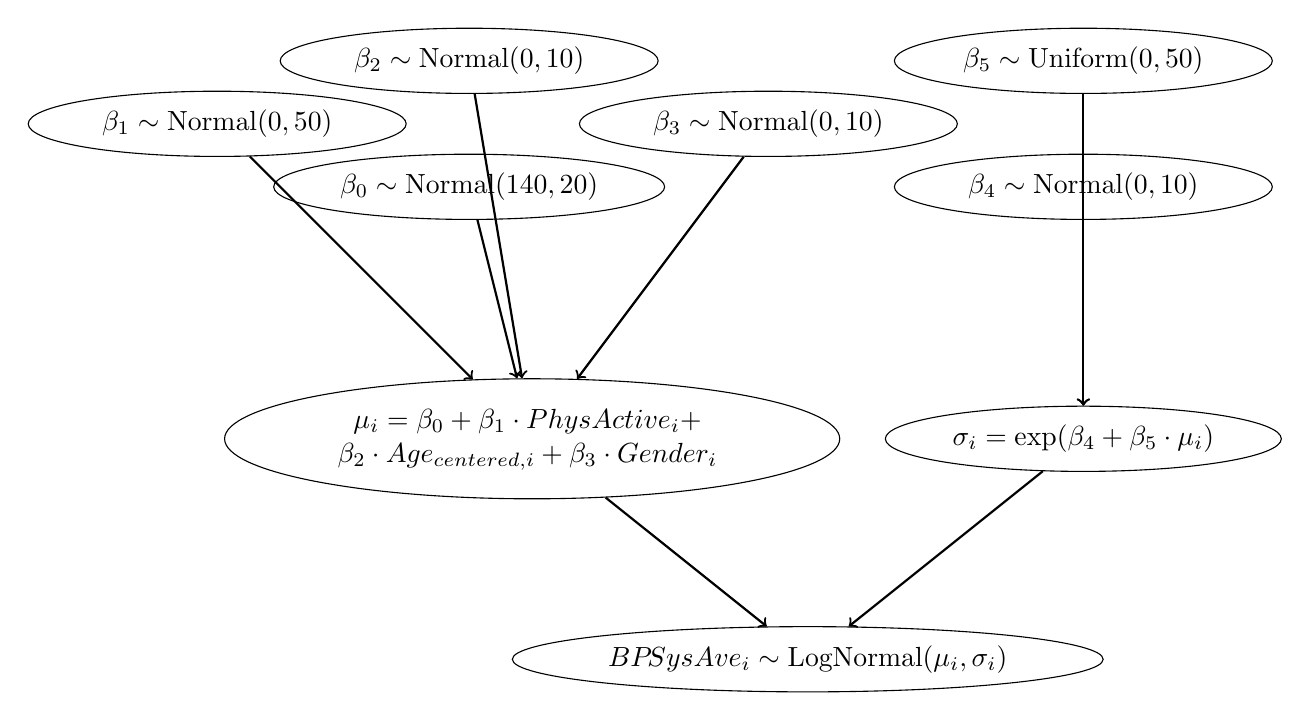
\begin{tikzpicture}[
    node distance=1.8cm and 3.2cm,
    every node/.style={draw, ellipse, align=center, font=\normalsize, minimum width=4.8cm}
]

% Priors
\node (b1) at (-6, 4) {\(\beta_1 \sim \mathrm{Normal}(0, 50)\)};
\node (b0) at (-2.8, 3.2) {\(\beta_0 \sim \mathrm{Normal}(140, 20)\)};
\node (b2) at (-2.8, 4.8) {\(\beta_2 \sim \mathrm{Normal}(0, 10)\)};
\node (b3) at (1, 4) {\(\beta_3 \sim \mathrm{Normal}(0, 10)\)};
\node (b4) at (5, 3.2) {\(\beta_4 \sim \mathrm{Normal}(0, 10)\)};
\node (b5) at (5, 4.8) {\(\beta_5 \sim \mathrm{Uniform}(0, 50)\)};

% Mu mit array für Zeilenumbruch
\node (mu) at (-2, 0) {
  $\begin{array}{c}
  \mu_i = \beta_0 + \beta_1 \cdot PhysActive_i + \\
  \beta_2 \cdot Age_{centered,i} + \beta_3 \cdot Gender_i
  \end{array}$
};

% Sigma daneben
\node (sigma) at (5, 0) {\(\sigma_i = \exp(\beta_4 + \beta_5 \cdot \mu_i)\)};

% Ergebnis unten
\node (obs) at (1.5, -2.8) {\(BP\!SysAve_i \sim \mathrm{LogNormal}(\mu_i, \sigma_i)\)};

% Pfeile zu mu
\draw[->, thick] (b0) -- (mu);
\draw[->, thick] (b1) -- (mu);
\draw[->, thick] (b2) -- (mu);
\draw[->, thick] (b3) -- (mu);

% Pfeile zu sigma
\draw[->, thick] (b4) -- (sigma);
\draw[->, thick] (b5) -- (sigma);

% Pfeile zur Beobachtung
\draw[->, thick] (mu) -- (obs);
\draw[->, thick] (sigma) -- (obs);

\end{tikzpicture}

\end{document}